\section{Error en la aproximación de Padé}

\subsection{Problema}
En relación a la función de ajuste $D(t)$ calculada por mínimos cuadrados, obtenga la funcióde error absoluto que se comete con el aproximante de Padédel apartado a) calculado alrededor de tres puntos distintos $t_0 = 1.0$, $t_0 = 1.5$ y $t_0 = 2.0$ y para los valores $\alpha$ y $\beta$ calculados en el ajuste. Calcule el error cuadrático en todos los casos y discuta la bondad de los ajustes.


\subsection{Resolución}

El código que se ha usado en la resolución de este problema está en \ref{code:ex6}. Se puede ver gráficamente el error absoluto de las tres aproximaciones en respecto al ajuste de mínimos cuadrados.

\begin{figure}[H]
	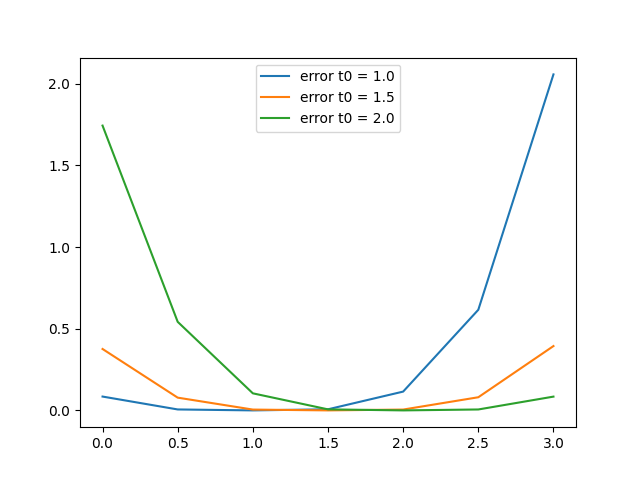
\includegraphics[width=\linewidth]{figures/error_abs_pade.png}
	\caption{Error de las aproximaciones de Padé en respecto al ajuste de mínimos cuadrados.}
	\label{fig:error_abs_pade}
\end{figure}

\newpage 

\paragraph{Valores}

Los valores son:

\begin{itemize}
	\item error $t_0 = 1.0 = 2.885144$
	\item error $t_0 = 1.5 = 0.938547$
	\item error $t_0 = 2.0 = 2.486423$
\end{itemize}

\subsection{Discusión}

Como se puede ver en la gráfica, es bastante importante asegurarnos de realizar la aproximación de Padé centrada en el intervalo de interés. Si sólo queremos calcular una aproximación, podemos ver que tomando el $t_0$ más céntrico ($1.5$), da un error bastante aceptable (una orden de magnitud de diferencia!).